% ====chapter=====
\myChapter{Un benchmark d’évaluation de la composition incrémentale des services}{}
\label{chap:contribution}
\myMiniToc{mysection}{Sommaire}

\mySection{Introduction}{}
% Ce chapitre propose un benchmark complet fondé sur la transformée de Fourier Rapide (FFT), dont l’architecture \textit{Diviser–Récursion–Combiner} s’intègre naturellement dans un modèle GAG. Il décrit la conception, l’implémentation et l’évaluation expérimentale, afin de démontrer comment la composition incrémentale améliore la latence, le parallélisme et la modularité, comparativement à un déploiement non incrémental.

À l'issue d’une revue approfondie de la littérature sur la composition incrémentale présentée dans le chapitre précédent, il apparaît clairement que, si les moteurs basés sur les Grammaires Attribuées Gardées (GAG) ont démontré leur faisabilité — \textit{notamment à travers un prototype de tri récursif} \cite{tagueu2024service} —, leur impact concret sur la performance reste à quantifier. %Les benchmarks existants s’appuient essentiellement sur des charges de travail simples et des déploiements statiques, sans jamais mesurer ni la réduction de la latence ni l’amélioration du parallélisme permises par une exécution « paresseuse ».

% Dans ce chapitre, nous proposons un protocole de benchmarking inédit fondé sur la transformée de Fourier Rapide (FFT). Choisie pour son utilisation répandue et sa complexité $\mathcal{O}(nlogn)$. Sa structure naturelle \textit{Diviser–Récursion–Combiner} constitue un cas d’étude idéal. Elle permet de modéliser chaque phase de calcul en microservices conteneurisés, orchestrés dynamiquement par Kubernetes et déclenchés selon des règles GAG ou un algorithme F qui suit le schéma : « diviser » → « multiples récursions sur F » → « combinaison ». Chaque étape peut être modélisée par un microservice déployé sur un conteneur, transformant ainsi le schéma en : « appel du service de division » → « multiples appels de service sur F » → « appel du service de combinaison ».
Dans ce chapitre, nous proposons un protocole de \textit{benchmarking} basé sur la transformée de Fourier Rapide (FFT). Ce choix se justifie par sa large utilisation dans des domaines tels que le traitement du signal ou les communications numériques, ainsi que par sa complexité algorithmique bien connue, en $\mathcal{O}(n \log n)$. La FFT suit une structure naturelle de type \textit{Diviser–Récursion–Combiner}, qui en fait un cas d’étude idéal pour évaluer la composition incrémentale de services.

Chaque phase de cet algorithme peut être modélisée comme un microservice indépendant, déployé dans un conteneur Docker et orchestré dynamiquement par Kubernetes. L'exécution est pilotée par un moteur basé sur les Grammaires Attribuées Gardées (GAG) ou, plus généralement par tout algorithme récursif $F$ suivant le schéma : « diviser » $\rightarrow$ « appels récursifs sur $F$ » $\rightarrow$ « combinaison ». Ce paradigme se traduit concrètement par une exécution distribuée : « appel du service de division » $\rightarrow$ « appels multiples de services récursifs sur $F$ » $\rightarrow$ « appel du service de combinaison ». Cette modélisation permet de tirer pleinement parti des capacités d'exécution paresseuse et parallèle de la composition incrémentale.

L’objectif de ce chapitre est double : d’une part, établir une méthodologie rigoureuse — \textit{de la mise en place des services FFT à la collecte des métriques de parallélisme, robustesse et scalabilité} —, et d’autre part, comparer de manière empirique l’approche incrémentale à un déploiement non incrémental. Grâce à ce benchmark reproductible, nous visons à quantifier précisément les gains de performance offerts par la composition incrémentale et à dégager des recommandations pratiques pour l’exploitation de ces moteurs sur des infrastructures hétérogènes.%CPU/GPU hétérogènes.

\mySection{Mise en place de la solution}{}
Dans cette section, nous présentons la démarche adoptée pour modéliser et déployer une version distribuée et paresseuse de l’algorithme FFT en nous appuyant sur les GAG. L’objectif est de mettre en œuvre une composition incrémentale fondée sur le paradigme classique \textit{Diviser – Récursion – Combiner}, où chaque étape du calcul est encapsulée dans un service distinct.

Bien que des algorithmes FFT bien établis permettent d’obtenir une complexité en temps de l’ordre de $\mathcal{O}(n \log n)$, ils se heurtent à une difficulté majeure dans les contextes applicatifs modernes : \textit{la gestion de grandes quantités de données}. Pour pallier ce problème, plusieurs implémentations parallèles ont été proposées, afin de tirer parti du parallélisme matériel. Cependant, ces approches restent souvent réservées aux utilisateurs disposant de ressources matérielles spécifiques (notamment des cartes graphiques hautes performances).

Dans cette optique, les implémentations distribuées de la FFT se révèlent particulièrement adaptées : elles permettent de répartir les calculs sur plusieurs nœuds interconnectés et de mieux exploiter les infrastructures modernes de calcul, comme les clusters cloud. En adoptant une approche basée sur les GAG, nous visons à rendre la FFT distribuée à la fois plus modulaire, plus flexible, et surtout plus accessible — même à des utilisateurs ne disposant que d’infrastructures standards.

\subsection{Approche méthodologique}{}

L’algorithme FFT suit une approche classique \textit{DPR}. Un vecteur d’entrée $x$ de taille $N = 2^k$ est divisé en deux sous-vecteurs : l’un regroupant les éléments d’indice pair, l’autre ceux d’indice impair. Chacun de ces sous-vecteurs est ensuite traité récursivement par la même fonction, jusqu’à atteindre le cas de base, où le vecteur ne contient qu’un ou deux éléments. À ce stade, le calcul peut être réalisé directement à l’aide de la formule de la DFT.

Dans le cas général, chaque appel récursif renvoie la transformée (FFT) de son sous-vecteur. Ces deux résultats intermédiaires sont ensuite combinés selon la formule bien connue :
\[
X[k] = E[k] + W_N^k \cdot O[k] \quad \text{et} \quad X[k + N/2] = E[k] - W_N^k \cdot O[k]
\]
où $E$ et $O$ représentent respectivement les FFT du sous-vecteur pair et impair, et $W_N^k$ la $k$-ième racine $N$-ième de l’unité. Ce découpage naturel rend l’algorithme hautement parallélisable, les sous-transformées pouvant être calculées indépendamment.

notre approche exploite cette propriété en encapsulant chaque appel récursif dans un service autonome. La fonction FFT est ainsi implémentée comme un microservice conteneurisé, déployé au sein d’un cluster Kubernetes. L’orchestrateur est chargé d’assigner dynamiquement les appels récursifs aux nœuds disponibles, en fonction de la charge du système. Une API REST permet la communication entre les différentes instances, assurant la sérialisation des données et la coordination du calcul distribué.

Cependant, cette architecture classique introduit une dépendance forte entre les services: \textit{la combinaison finale des résultats requiert que les deux sous-transformées soient disponibles simultanément}. Une panne sur l’un des deux services bloque donc le processus, ce qui limite la résilience globale de l’application.

Pour atténuer cette contrainte, nous proposons une variante incrémentale et paresseuse de la FFT distribuée, fondée sur les GAG. L’idée est de diviser le signal initial en $k$ blocs élémentaires, chacune étant confiée à un service FFT. À chaque appel récursif, ces blocs peuvent être divisées localement en sous-blocs (paires et impaires), puis traitées indépendamment.

Une fois les résultats disponibles, la combinaison peut s’effectuer dès que deux blocs transformées sont prêtes, sans attendre l’ensemble du signal. Cela permet à l’algorithme de produire des résultats partiels au fil de l’eau. En cas de panne d’un service, le système peut continuer à traiter les blocs disponibles et combiner progressivement les résultats, réduisant ainsi les effets de blocage.

Cette stratégie améliore sensiblement la tolérance aux pannes, au prix d'un léger surcoût computationnel, tout en s’inscrivant naturellement dans une logique de composition incrémentale distribuée. Elle met à profit les capacités expressives des GAG pour orchestrer dynamiquement les étapes du calcul selon les dépendances effectives entre les blocs.

\textbf{Pseudocode de la FFT paresseuse.}
Dans notre approche, le vecteur d’entrée est découpé en blocs élémentaires appelés \textit{cellules}. Chaque cellule est traitée indépendamment par un service, qui effectue la transformation sur un petit sous-ensemble de données.

Les résultats partiels ainsi produits (sous-cellules combinées) sont ensuite combinés par des services intermédiaires selon la structure récursive de la FFT. Chaque service peut être déclenché dès que deux cellules transformées sont disponibles, permettant une exécution asynchrone, incrémentale et tolérante aux pannes. Le traitement se poursuit jusqu’à ce que le service racine obtienne le spectre complet.

% Les résultats partiels ainsi produits sont ensuite combinés progressivement par des services intermédiaires (\texttt{RecFFT}) selon la structure récursive de la FFT. Chaque service peut être déclenché dès que deux cellules transformées sont disponibles, permettant une exécution asynchrone, incrémentale et tolérante aux pannes. Le traitement se poursuit jusqu’à ce que le service racine (\texttt{MainFFT}) obtienne le spectre complet.

Cette logique peut être exprimée par un pseudocode simplifié, illustrant la récursivité et la production partielle des résultats (Algo. \ref{alg:lazy_fft}):

% \begin{algorithm}[H]
% \DontPrintSemicolon
% \KwIn{Signal d'entrée et \texttt{blocSize} blocs}
% \KwOut{Résultat de la FFT paresseuse}

% \If{taille du signal $\leq$ seuil}{
%     Appliquer \texttt{BaseFFT} sur chaque bloc\;
%     \Return résultats FFT\;
% }

% Découper le signal en \texttt{blocSize} blocs de taille égale\;

% \For{chaque bloc}{
%     Séparer les éléments pairs et impairs pour former \texttt{evenBlocs} et \texttt{oddBlocs}\;
% }
% % Former \texttt{evenBlocs} et \texttt{oddBlocs}\;

% Appeler récursivement \texttt{FFT\_lazy(evenBlocs)} et \texttt{FFT\_lazy(oddBlocs)}\;

% \For{chaque couple de blocs $(even_k, odd_k)$ disponible}{
%     Combiner les deux pour produire un bloc FFT\;
%     \If{le bloc est complet \textbf{et} le service courant $\neq$ racine}{
%         Transmettre le bloc au parent\;
%     }
% }

% \caption{Algorithme FFT Paresseux}
% \end{algorithm}
\begin{algorithm}[H]
\DontPrintSemicolon
\KwIn{Signal d'entrée \texttt{x}, nombre de blocs \texttt{blocSize}}
\KwOut{Résultat partiel ou complet de la FFT paresseuse}

\If{taille(\texttt{x}) $\leq$ seuil}{
    appliquer \texttt{BaseFFT}$(x)$\;
    % \For{chaque bloc $b$ dans \texttt{x}}{
    % }
    % \Return résultats FFT des blocs\;
}

Découper \texttt{x} en \texttt{blocSize} blocs de taille égale\;

\For{chaque bloc}{
    séparer les éléments d'indice pair et impair\;
    former deux listes : \texttt{evenBlocs} et \texttt{oddBlocs}\;
}

$E \gets$ \texttt{FFT\_lazy(evenBlocs)}\;
$O \gets$ \texttt{FFT\_lazy(oddBlocs)}\;

\For{chaque couple $(E_k, O_k)$ disponible}{
    $X_k \gets E_k + W^k \cdot O_k$\;
    $X_{k+N/2} \gets E_k - W^k \cdot O_k$\;
    
    \If{bloc $X$ est complet \textbf{et} le service courant $\neq$ racine}{
        transmettre $X$ au parent\;
    }
}

\caption{Algorithme FFT Paresseux}
\label{alg:lazy_fft}
\end{algorithm}

\vspace{1cm}

Cette logique est ensuite traduite en règle GAG, dans laquelle chaque opération de l’algorithme devient une règle autonome, pouvant être exécutée indépendamment des autres. 
Grâce à l’abstraction offerte par le modèle, l’exploitation du parallélisme dans un environnement distribué devient transparente pour le développeur :
le moteur GAG se charge de gérer l’expansion du graphe de composition, tandis que l’orchestrateur (Kubernetes) alloue dynamiquement les ressources en fonction de la charge, garantissant ainsi une exécution optimisée sans effort manuel supplémentaire.

Notre conception distingue deux types complémentaires de services :
\begin{itemize}
    \item \textbf{Les services internes}, interprétés directement par le moteur GAG, correspondent aux symboles non terminaux de la grammaire. Ils définissent la structure logique du traitement à réaliser (décomposition, appels récursifs, combinaison, etc.);
    \item \textbf{Les services externes}, quant à eux, sont gérés par l’orchestrateur. Il s’agit des entités concrètes déployées dans le cluster (sous forme de pods), et que l’application peut invoquer dynamiquement via API REST.
\end{itemize}

Pour assurer un couplage cohérent entre ces deux couches (\textit{logique et infrastructurelle}), chaque service interne est associé à une entrée explicite dans le fichier de spécification YAML. Ce fichier décrit le nom du service, ses entrées et sorties, ses gardes éventuelles, les sous-services enfants, ainsi que la correspondance entre les attributs.

Trois services fondamentaux émergent de cette modélisation :
\begin{itemize}
  \item \textbf{MainFFT} : service racine qui initie le calcul ; il décompose le signal d’entrée en blocs, délègue le traitement au service récursif, puis combine les résultats obtenus ;
  \item \textbf{RecFFT} : service récursif qui applique la logique de division des blocs et d’appels imbriqués ;
  \item \textbf{CombineFFT} : service qui se charge de la combinaison de deux blocs.
\end{itemize}

Chaque règle GAG est associée à des attributs (entrées, sorties) et activée sous condition (garde). Ce formalisme permet de représenter explicitement les dépendances de données, et d’exécuter le calcul de manière progressive, distribuée et faiblement synchronisée, tout en garantissant la cohérence finale du résultat.
\vspace{0.5cm}
\begin{lstlisting}[caption={Declaration des Services}, label={lst:services}]
# Service principal : lance la composition FFT sur le signal complet
---
kind: service
name: MainFFT
kubename: ${KUBE_NAME}
inputs:
  - { name: in_signal, array: true, size: ${NUMBER_OF_BLOCKS} }
outputs:
  - { name: spectrum }
  
# Service récursif : divise le signal en sous-blocs et les traite récursivement
---
kind: service
name: RecFFT
kubename: ${KUBE_NAME}
inputs:
  - { name: signal, array: true, size: ${NUMBER_OF_BLOCKS} }
outputs:
  - { name: spectrum, array: true, size: ${NUMBER_OF_BLOCKS} }
  
# Service de combinaison : combine les parties paires et impaires après FFT
---
kind: service
name: CombineFFT
kubename: ${KUBE_NAME}
inputs:
  - { name: even, array: true, size: ${NUMBER_OF_BLOCKS} }
  - { name: odd, array: true, size: ${NUMBER_OF_BLOCKS} }
outputs:
  - { name: output }
\end{lstlisting}

Chaque service possède un champ \texttt{name} (listing \ref{lst:services}, ligne 4) qui correspond au nom du service interne, c’est-à-dire à la règle interprétée par le moteur GAG. Le champ \texttt{kubename} (listing \ref{lst:services}, ligne 5), quant à lui, représente le nom du service externe tel qu’il est connu de l’orchestrateur Kubernetes, et permet son invocation effective au moment du déploiement.
% Cette logique est ensuite traduite en une grammaire GAG dans laquelle chaque opération devient une règle autonome, pouvant être exécutée indépendamment des autres.  
% On identifie trois services fondamentaux :
% \begin{itemize}
%   \item \textbf{MainFFT}: service racine qui initie le calcul, il décompose le signal d’entrée en blocs, le passe aux service récursif puis combine le résultat;
%   \item \textbf{RecFFT}: service récursif qui applique la logique de division et d’appel;
%   \item \textbf{BaseFFT}: service de terminaison qui exécute localement la DFT.
% \end{itemize}

% Chaque règle GAG est dotée de ses propres attributs (paramètres d’entrée et de sortie) et s’active lorsque sa garde est satisfaite. Cette modélisation rend possible une exécution progressive, distribuée et faiblement synchronisée du calcul FFT, tout en assurant la cohérence globale du résultat.

\subsection{Architecture du prototype}{}
%%%%%%%%% Draft %%%%%%%%%%
% \section*{Architecture du prototype}
% Le prototype repose sur une chaîne de traitement en trois étapes principales (voir Figure 1) :
Le prototype de notre solution, initialement mis en œuvre dans \cite{tagueu2024service} lors de l’implémentation du tri incrémental, repose sur une chaîne de traitement en trois étapes principales (Figure \ref{fig:archi-prototype}) :

\begin{figure}[h]
    \centering
    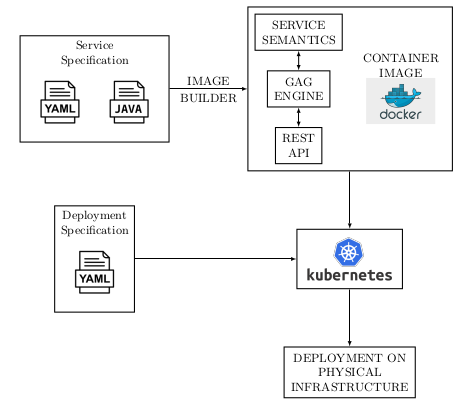
\includegraphics[width=0.7\linewidth]{My-Thesis/Chap3/images/Architecture.png}
    \caption{Architecture du prototype \cite{tagueu2024service}}
    \label{fig:archi-prototype}
\end{figure}

\begin{enumerate}
\item \textbf{Spécification de service :} un fichier YAML décrit la composition des services, incluant la déclaration de services externes et l’appel à des fonctions locales implémentées en Java. Ce langage de description permet de définir des services composites fondés sur les GAG;
\item \textbf{Construction de l'image Docker :} l’\emph{Image Builder} compile les spécifications YAML et le code Java pour produire la sémantique de service interprétable par le moteur GAG. Cette sémantique, le moteur GAG et une API REST sont empaquetés dans un conteneur Docker unique;
\item \textbf{Orchestration Kubernetes :} à partir d'un second fichier YAML définit la spécification de déploiement, Kubernetes déploie alors chaque conteneur sur un cluster, gérant automatiquement l’allocation des ressources, la montée en charge et la tolérance aux pannes.
\end{enumerate}
% À l’exécution, le moteur GAG orchestre les appels aux microservices FFT de façon paresseuse : chaque phase (division, récursions, combinaison) est déclenchée uniquement si ses données d’entrée sont disponibles, optimisant ainsi la latence et le parallélisme.
%%%%%%%%% Draft %%%%%%%%%%

% \subsection{Architecture du système}{}
% On y décrit les phases du projet : fondations théoriques, modélisation de la solution, et expérimentation via déploiement sur une infrastructure conteneurisée et orchestrée.

\subsection{Processus de déploiement de l'algorithme}{}
% Cette sous-section détaille la manière dont l’algorithme FFT a été implémenté sous forme de microservices distribués. Elle décrit le workflow d’exécution, depuis la décomposition initiale du signal jusqu’à la combinaison des résultats partiels, en s’appuyant sur le modèle Diviser–Récursion–Combiner. L'enchaînement des services conteneurisés est orchestré dynamiquement par Kubernetes, tandis que l’exécution est pilotée par le moteur GAG selon les règles spécifiées dans les fichiers YAML. L’objectif ici est d’expliquer comment la logique FFT a été traduite en une architecture modulaire, distribuée et pilotée paresseusement.

% L’approche que nous utilisons permet de transformer un algorithme classique exprimé sous forme récursive en une composition de services paresseux. L’activation incrémentale des règles est pilotée par les dépendances de données, ce qui permet une exécution progressive, distribuée et résiliente, tout en conservant la logique algorithmique initiale.

% Grâce à l’abstraction offerte par le modèle, l’exploitation du parallélisme dans un environnement distribué devient transparente pour le développeur :
% le moteur GAG se charge de gérer l’expansion du graphe de composition, tandis que l’orchestrateur (Kubernetes) alloue dynamiquement les ressources en fonction de la charge, garantissant ainsi une exécution optimisée sans effort manuel supplémentaire.
\textbf{Production.}
La sémantique associée à chaque service est définie par la \textbf{règle de production} qui lui est liée.
Lorsque le service n’est pas décomposable en plusieurs alternatives, il est nécessaire de lui associer une garde. Cette garde est généralement une fonction qui retourne toujours la valeur \textit{true}, indiquant que la règle est toujours applicable pour résoudre le service. Elle joue un rôle formel pour satisfaire le schéma de la grammaire, même si elle ne conditionne pas réellement l’activation de la règle.

La section \texttt{functions} (listings \ref{lst:main_pdtion}, ligne 8) permet de déclarer les \textit{fonctions locales} utilisées par la règle, et chaque fonction peut être identifiée par un alias via le champ \texttt{label} (listings \ref{lst:main_pdtion}, lignes 10, 12). Ces alias facilitent ensuite leur utilisation dans la section \texttt{actions} (listings \ref{lst:main_pdtion}, ligne 13), qui décrit les règles sémantiques de la production.\\

\begin{lstlisting}[caption={Production du service MainFFT}, label={lst:main_pdtion}]
---
kind: rule
name: Main_FFT
service: MainFFT
guard:
  classPath: com.local.FourierFunc
  method: checklength
functions:
  - { classPath: com.local.FourierFunc, method: split,
        label: split, multiOutput: true, outputSize: ${NUMBER_OF_BLOCKS} }
  - { classPath: com.local.FourierFunc, method: combine_f,
        label: combine }
actions:
  - blocks = split(in_signal)
  - result_blocks = RecFFT(blocks)
  - half1 = CombineFFT(result_blocks[0], result_blocks[1])
  - half2 = CombineFFT(result_blocks[2], result_blocks[3])
  - spectrum = combine(half1, half2)
\end{lstlisting}
% \begin{verbatim}
% ---
% kind: rule
% name: Main_FFT
% service: MainFFT
% guard:
%   classPath: com.local.FourierFunc
%   method: checklength
% functions:
%   - { classPath: com.local.FourierFunc, method: split,
%         label: split, multiOutput: true,
%         outputSize: ${NUMBER_OF_BLOCKS} }
%   - { classPath: com.local.FourierFunc, method: combine_f,
%         label: combine }
% actions:
%   - blocks = split(in_signal)
%   - result_blocks = RecFFT(blocks)
%   - half1 = CombineFFT(result_blocks[0], result_blocks[1])
%   - half2 = CombineFFT(result_blocks[2], result_blocks[3])
%   - spectrum = combine(half1, half2)
% \end{verbatim}
% \vspace{-0.5cm}\hspace{2cm} Production du service MainFFT\\

\begin{lstlisting}[caption={Une des productions du service RecFFT}]
---
kind: rule
name: Rec_FFT_remote
service: RecFFT
guard:
  classPath: com.local.FourierFunc
  method: checklength_in
functions:
  - { classPath: com.local.FourierFunc, method: divide, 
      label: divide, multiOutput: true, outputSize: ${NUMBER_OF_BLOCKS} }
actions:
  - part1, part2 = divide(signal)
  - res1 = RecFFT(part1)
  - res2 = RecFFT(part2)
  - out1 = CombineFFT(res1[0], res1[1])
  - out2 = CombineFFT(res1[2], res1[3])
  - out3 = CombineFFT(res2[0], res2[1])
  - out4 = CombineFFT(res2[2], res2[3])
  - spectrum = [out1, out2, out3, out4]
\end{lstlisting}
% \begin{verbatim}
% ---
% kind: rule
% name: Rec_FFT
% service: RecFFT
% guard:
%   classPath: com.local.FourierFunc
%   method: checklength_in
% functions:
%   - { classPath: com.local.FourierFunc, method: divide, 
%         label: divide, multiOutput: true, 
%         outputSize: ${NUMBER_OF_BLOCKS} }
% actions:
%   - part1, part2 = divide(signal)
%   - res1 = RecFFT(part1)
%   - res2 = RecFFT(part2)
%   - out1 = CombineFFT(res1[0], res1[1])
%   - out2 = CombineFFT(res1[2], res1[3])
%   - out3 = CombineFFT(res2[0], res2[1])
%   - out4 = CombineFFT(res2[2], res2[3])
%   - spectrum = [out1, out2, out3, out4]
% \end{verbatim}
% \vspace{-0.5cm}\hspace{2cm} Une des productions du service RecFFT\\

\begin{lstlisting}[caption={Production du service CombineFFT}, label={lst:combine_pdtion}]
---
kind: rule
name: Combine
service: CombineFFT
guard:
  classPath: com.local.FourierFunc
  method: combine_guard
functions:
  - { classPath: com.local.FourierFunc, method: twiddle_combine,
      label: twiddle_combine }
actions:
  - output = twiddle_combine(even, odd)
\end{lstlisting}
% \begin{verbatim}
% ---
% kind: rule
% name: Combine
% service: CombineFFT
% guard:
%   classPath: com.local.FourierFunc
%   method: combine_guard
% functions:
%   - { classPath: com.local.FourierFunc, method: twiddle_combine,
%         label: twiddle_combine }
% actions:
%   - output = twiddle_combine(even, odd)
% \end{verbatim}
% \vspace{-0.5cm}\hspace{2cm} Production du service CombineFFT\\

Le déploiement de l’algorithme s’appuie sur un environnement distribué simulé localement à l’aide de machines virtuelles. Pour cela, nous utilisons %le dossier \texttt{Cluster}, 
un dossier qui regroupe l’ensemble des ressources nécessaires à la création du cluster. Celui-ci est généré à l’aide des outils Vagrant\cite{hashicorp_vagrant_docs} et VirtualBox\cite{virtualbox}. Chaque machine virtuelle agit comme un nœud logique du cluster.

\textbf{Compilation des services.}
% Avant de pouvoir déployer les services, il est nécessaire de générer une image Docker pour chacun d’entre eux. Cette image contient tous les éléments nécessaires à son exécution autonome a savoir le code compile du moteur GAG et les fichiers de spécifications des services (au format YAML) décrivant la structure, les règles de productions, les gardes associees ainsi que les fonctions locales (que l'on implemente en Java).
% Ces éléments sont compilés et regroupés à l’aide d’un outil interne de construction d’image. Les binaires ainsi générés sont embarqués dans l’image Docker, accompagnés des fichiers de description. En théorie, les fichiers de règles pourraient être précompilés en structures internes optimisées, mais dans le cadre de notre prototype, cette analyse est effectuée dynamiquement au moment de l’exécution, par le moteur GAG lui-même.
Avant de pouvoir déployer les services, il est nécessaire de générer une image Docker pour chacun d’entre eux. Chaque image regroupe l’ensemble des éléments nécessaires à l’exécution autonome du service concerné. Cela inclut :

\begin{itemize}
  \item le code compilé du moteur GAG, responsable de l’interprétation et de l’évaluation des règles de composition ;
  \item les fichiers de spécification des services, écrits en YAML, définissant la structure du service, ses attributs, ses dépendances et ses sous-services ;
  \item les règles de production, également spécifiées en YAML, décrivant les conditions de déclenchement (gardes) et les actions associées ;
  \item les fonctions locales implémentées en Java, utilisées pour effectuer des calculs ou manipulations internes spécifiques à chaque service.
\end{itemize}

L’ensemble de ces éléments est compilé et rassemblé à l’aide d’un outil de construction d’image interne. Ce dernier compile le code source, génère les binaires nécessaires, et assemble le tout dans une image Docker exécutable.

En principe, les fichiers de spécification et les règles pourraient être analysés à la compilation et traduits en structures internes prêtes à l’emploi. Toutefois, dans le cadre de ce prototype, cette analyse est volontairement déportée à l’exécution pour faciliter le développement et tester différentes configurations de manière souple. C’est donc le moteur GAG lui-même qui charge dynamiquement les règles au moment du lancement du conteneur.


\textbf{Déploiement sur le cluster Kubernetes.}
Une fois les images Docker créées, leur déploiement est orchestré à l’aide d’un fichier de spécification Kubernetes, rédigé au format YAML. Ce fichier référence les images construites et définit, pour chaque service :
\begin{itemize}
    \item les ressources nécessaires (CPU, mémoire, nombre de réplicas) ;
    \item les politiques de redémarrage, de tolérance aux pannes et d’équilibrage de charge ;
    \item les adresses ou ports d’exposition pour la communication REST.
\end{itemize}

L’exécution des commandes Kubernetes standard (telles que \texttt{kubectl apply}) suffit alors à déclencher le déploiement automatique des services sur les nœuds du cluster. Chaque image est instanciée sous forme de pod, et le moteur GAG contenu dans chaque conteneur pilote les appels de services à la volée, en fonction de l’état des données disponibles.

Ce processus garantit à la fois une gestion flexible du déploiement, une évolutivité naturelle via la déclaration du nombre de réplicas, et une robustesse améliorée par l’isolation des services.


\mySection{Conditions expérimentales}{}

\subsection{Environnement d’expérimentation}{}
% Cette sous-section décrit l’environnement matériel et logiciel utilisé pour évaluer les performances du prototype. Elle présente la configuration du cluster (nombre de nœuds, types de machines, disponibilité de GPU), les versions des outils déployés (Docker, Kubernetes, moteur GAG), ainsi que les outils de monitoring et de mesure. Elle précise également les ressources allouées à chaque conteneur (CPU/RAM) et les conditions de charge simulées.
L’environnement d’expérimentation mis en place dans le cadre de ce travail vise à évaluer les performances de la composition incrémentale sur des services distribués, modélisés à l’aide de Grammaires Attribuées Gardées (GAG). Pour assurer un déploiement contrôlé, reproductible et conforme aux scénarios d’exécution distribuée, nous avons opté pour une infrastructure virtualisée localement, articulée autour de conteneurs Docker et d’un cluster Kubernetes.

\textbf{Infrastructure de déploiement.} Les expérimentations ont été réalisées sur une machine personnelle moyenne de gamme avec un processeur Intel core i7 (4 cœurs, 2 threads) et une mémoire vive (RAM) de 8Go.

\textbf{Virtualisation et orchestration.} 
L’infrastructure distribuée a été simulée localement à l’aide de deux outils principaux :
\begin{itemize}
  \item \textit{Vagrant} : utilisé pour l’automatisation de la configuration et du provisionnement des machines virtuelles ;
  \item \textit{VirtualBox} : utilisé comme hyperviseur léger pour exécuter les VM localement.
\end{itemize}

Sur cette base, un cluster Kubernetes a été déployé manuellement, avec la configuration suivante :
\begin{itemize}
  \item \textit{1 nœud maître}: chargé de la gestion du plan de contrôle au sein du cluster;
  \item \textit{2 nœuds workers} : utilisés pour héberger et exécuter les services conteneurisés.
\end{itemize}

Chaque machine virtuelle dispose de :
\begin{itemize}
  \item \textit{2 vCPU} ;
  \item \textit{2048 Mo de RAM} pour le nœud maître ;
  \item \textit{1536 Mo de RAM} pour chaque nœud worker ;
  \item une adresse IP statique permettant la communication fluide entre les nœuds (consécutives à partir de 10.0.0.10).
\end{itemize}

\subsection{Paramètres de test}{}
% Les tests expérimentaux menés dans ce travail ont pour but d’évaluer la performance, la modularité, le parallélisme et la résilience du système reposant sur une composition incrémentale de services GAG, en comparaison avec une approche centralisée plus classique. Pour cela, plusieurs paramètres de test ont été définis et modifiés de manière systématique afin d’observer leurs effets sur le comportement de l’algorithme.
Les tests expérimentaux menés dans ce travail visent à évaluer les performances de la solution proposée selon plusieurs critères : \textbf{modularité}, \textbf{robustesse}, \textbf{capacité de parallélisation} et \textbf{résilience}. L’objectif est de comparer le comportement d’un système fondé sur la composition incrémentale de services avec celui d’une implémentation centralisée plus classique de l’algorithme FFT.

Pour cela, différents paramètres de test ont été définis et modifiés de manière systématique afin d’observer leur influence sur le déroulement du calcul et sur les performances obtenues.

\textbf{Taille du signal d’entrée.}
La taille du vecteur d’entrée soumis à la transformée de Fourier est un facteur clé dans l’analyse des performances. Les valeurs testées sont des puissances de 2, compatibles avec l’implémentation FFT récursive. Les tailles typiques testées vont de $N=2^{10}=1024$ à $N=2^{17}=131072$. Cette variation permet d’analyser la scalabilité du système et son comportement face à des volumes croissants de données.

\textbf{Seuil de découpage (bloc minimal).}
Un seuil est défini pour contrôler la granularité des blocs de données à partir desquels un service local applique la FFT de manière directe (algorithme naïf). Plus ce seuil est bas, plus la profondeur de l’arbre d’appels récursifs sera grande.
Cela permet d’étudier l'impact de la profondeur de récursion sur la performance globale et sur le niveau de parallélisme atteint.

\textbf{Niveau de parallélisme.}
Pour évaluer la capacité du système à exploiter le parallélisme offert par l’architecture distribuée, nous avons fait varier le nombre de pods déployés simultanément dans le cluster. Chaque pod exécute un ou plusieurs services dérivés des règles GAG, correspondant à une sous-tâche du traitement (séparation, FFT locale, combinaison, etc.).

Les configurations testées vont de 1 à 5 pods. Cette variation permet d’évaluer les gains de performance obtenus par la distribution des traitements FFT sur plusieurs conteneurs isolés.

Contrairement à une augmentation du nombre de nœuds physiques ou virtuels, cette approche contrôle le nombre d'instances de traitement logiques, tout en gardant constante l'infrastructure (nombre de nœuds Kubernetes). Elle est particulièrement adaptée pour tester l'efficacité de la gestion des ressources par l'orchestrateur (scheduler Kubernetes) et observer l'impact du niveau de composition des services sur les performances globales.

\mySection{Résultats et observations}{}
\subsection{Exécution distribuée}
Nous présentons dans cette section les résultats obtenus lors de l’évaluation expérimentale du système basé sur la composition incrémentale de services pour le calcul distribué de la transformée de Fourier rapide (FFT). L’objectif principal est d’analyser l’impact du parallélisme sur le temps d’exécution global, en fonction de la taille du signal en entrée.

\begin{figure}[h]
    \centering
    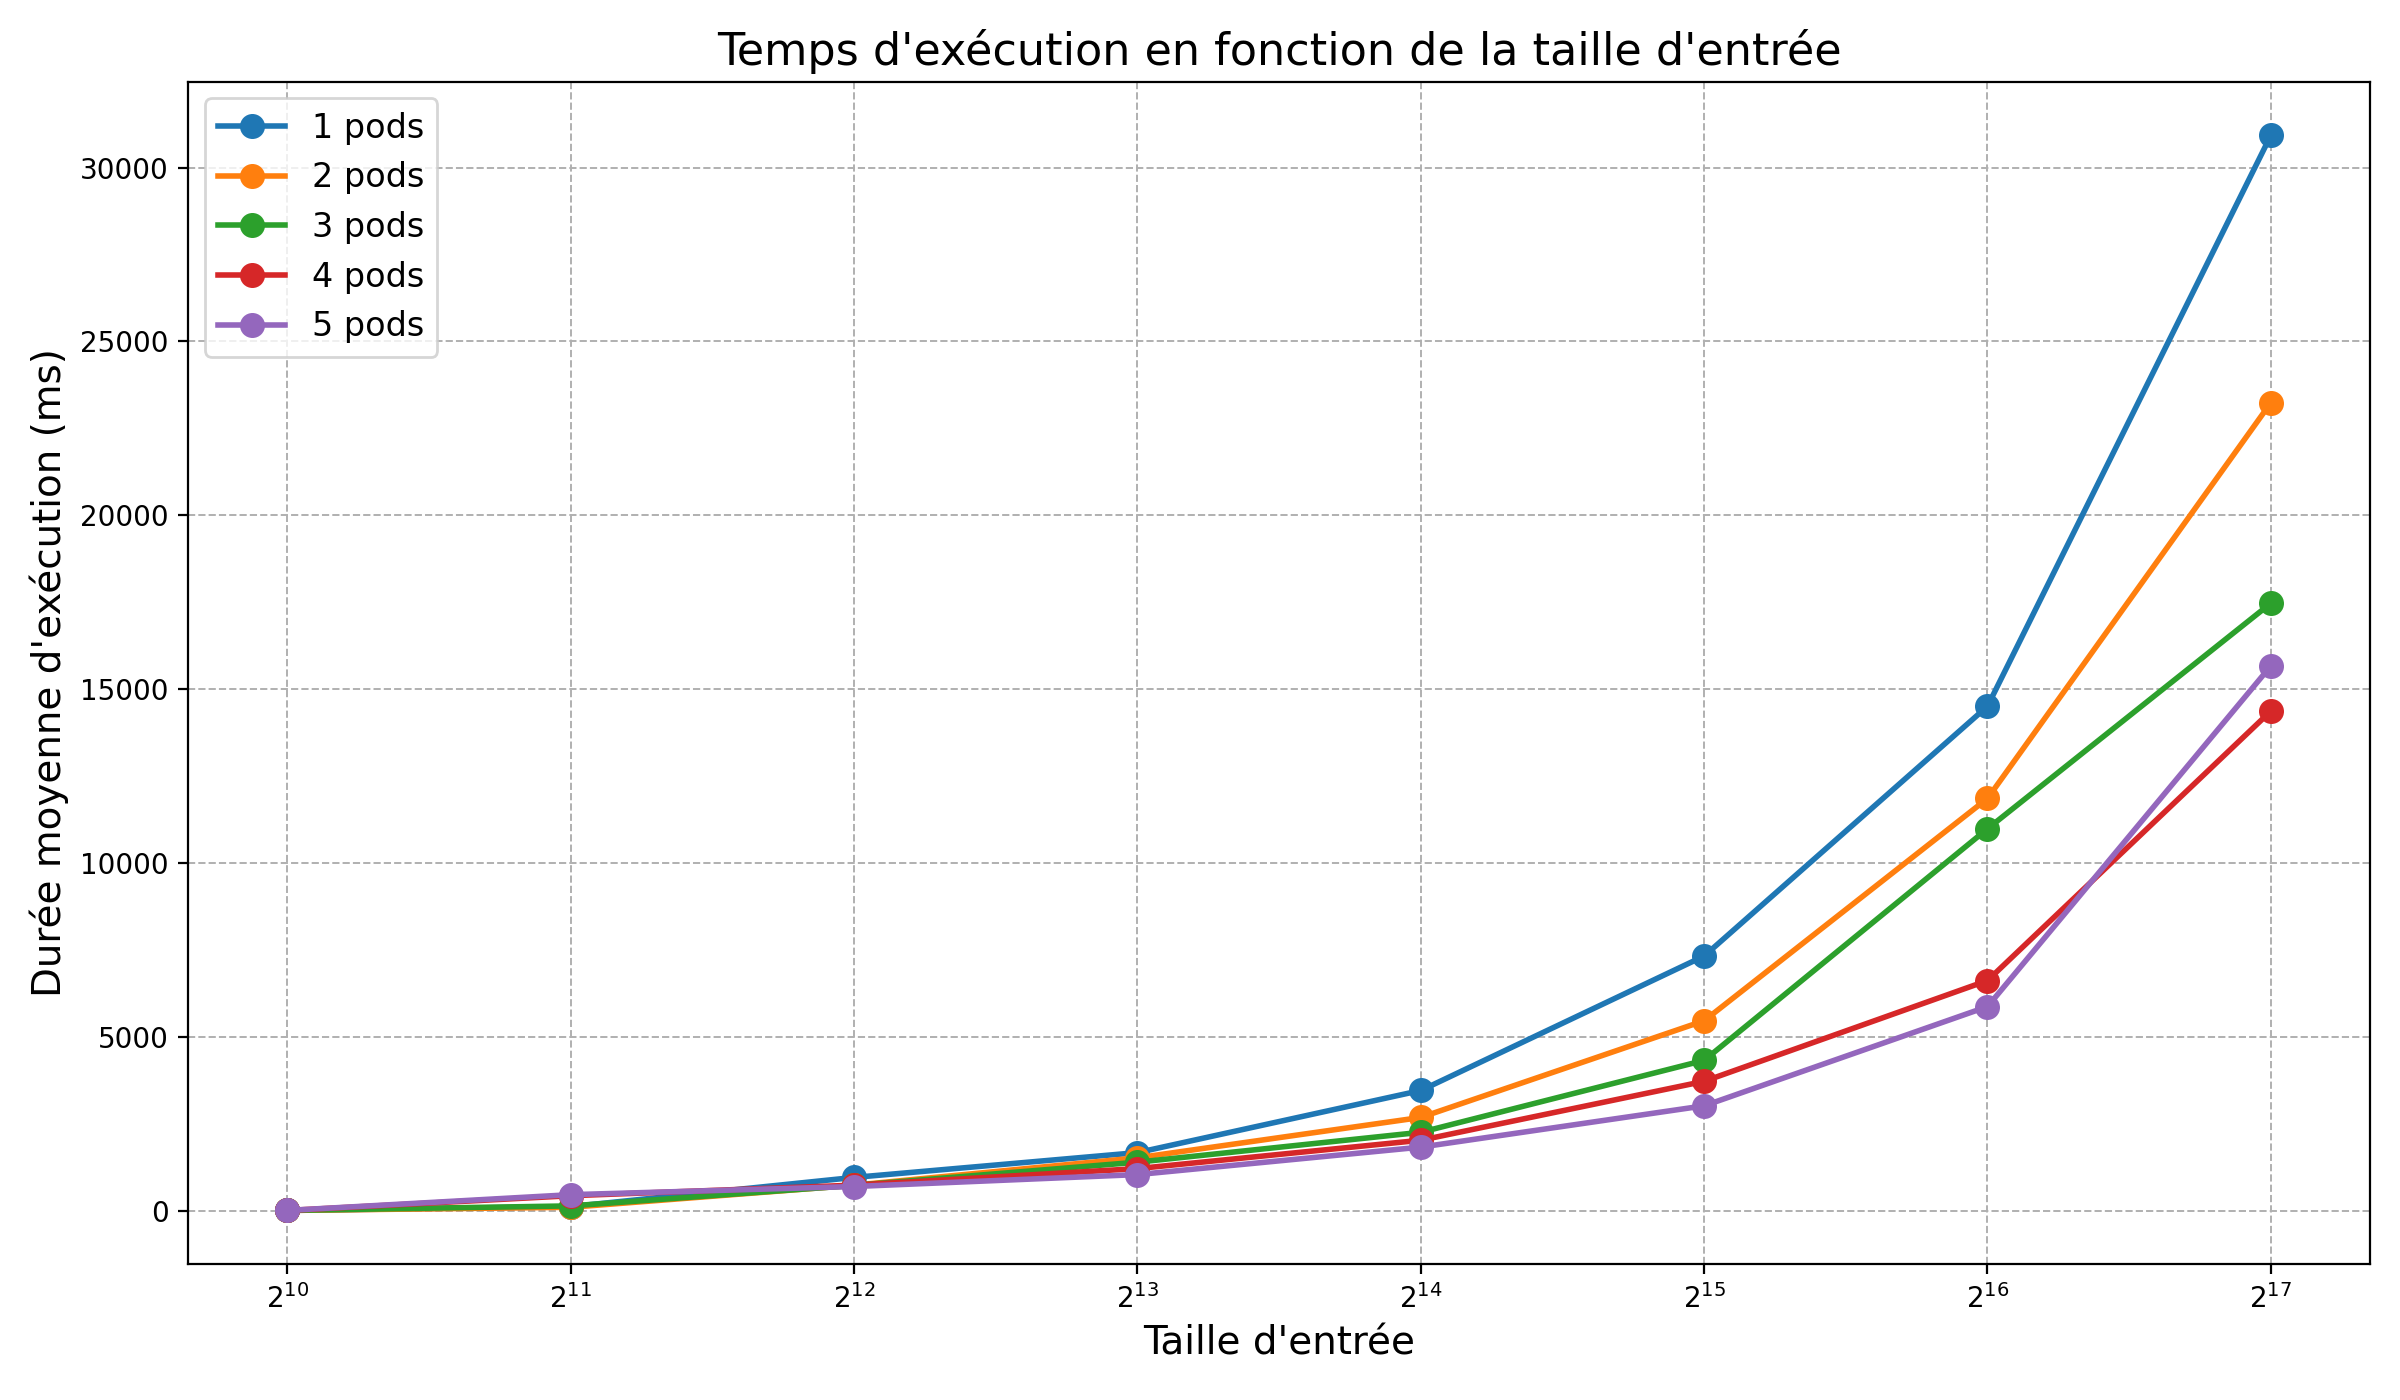
\includegraphics[width=\linewidth]{My-Thesis/Chap3/images/resultats-inc.png}
    \caption{Temps d’exécution moyen en fonction de la taille d’entrée pour différentes configurations de parallélisme}
    \label{fig:resultats-inc}
\end{figure}

\textbf{Analyse des performances.}
La Figure~\ref{fig:resultats-inc} illustre l’évolution du temps d’exécution moyen (en millisecondes) en fonction de la taille du signal d’entrée (en puissances de deux), pour des configurations comportant entre 1 et 5 pods actifs dans le cluster Kubernetes.

On observe les tendances suivantes :
\begin{itemize}
    \item Pour les petites tailles d’entrée ($2^{10}$ à $2^{13}$), les temps d’exécution restent relativement proches quelle que soit la configuration du cluster (de 1 à 5 pods). Cela s’explique par deux facteurs principaux.
    
    D’une part, la charge de calcul étant faible, le gain potentiel dû au parallélisme reste limité : la surcharge liée à la coordination et au déclenchement des services devient proportionnellement plus importante que le travail de transformation lui-même.
    
    D’autre part, l’architecture du système repose sur une communication interservices via une API REST, utilisant le protocole HTTP. À chaque appel de service, les blocs de données doivent être sérialisés, transmis sous forme de requêtes, puis désérialisés à la réception. Ce mécanisme introduit un surcoût fixe en temps.%, indépendant de la taille du signal. 
    
    Lorsque les entrées sont de taille réduite, ce coût de sérialisation/désérialisation devient prépondérant par rapport au temps de calcul effectif. Il en résulte une latence importante et un amortissement inefficace du coût d’invocation de service, rendant l’exécution parallèle moins avantageuse dans ces cas;
    
  % \item La configuration à 1 pod montre une croissance exponentielle du temps d’exécution, illustrant la difficulté à traiter efficacement des signaux volumineux sans parallélisme;
  
  \item À partir de $2^{14}$, l’impact du nombre de pods devient significatif. L’utilisation de plusieurs pods permet une meilleure répartition des calculs FFT sur les sous-tableaux, réduisant ainsi le temps total de traitement;

  % \item Pour les très grandes tailles ($2^{16}$ à $2^{17}$), le gain de performance apporté par l’augmentation du nombre de pods reste visible mais tend à se stabiliser. Le passage de 4 à 5 pods, par exemple, n’apporte qu’un bénéfice marginal. Cela suggère une saturation des ressources disponibles ou une surcharge liée à la coordination inter-pods;

  \item Pour les très grandes tailles d’entrée ($2^{16}$ à $2^{17}$), l’ajout de pods supplémentaires continue de réduire le temps d’exécution, mais les gains deviennent de plus en plus faibles. Par exemple, le passage de 4 à 5 pods n’apporte qu’un bénéfice marginal.

Ce phénomène s’explique principalement par une saturation des ressources physiques de la machine hôte. Le cluster étant simulé localement à l’aide de machines virtuelles, les performances globales dépendent directement de la capacité du système hôte (CPU, mémoire disponible). Or, à partir d’un certain niveau de parallélisme, toutes les ressources CPU et/ou mémoire sont déjà sollicitées. Le système n’est alors plus en mesure de répartir efficacement la charge supplémentaire.

Par ailleurs, plus le nombre de pods augmente, plus la coordination entre services devient coûteuse : échanges de messages, appels HTTP, sérialisation/désérialisation. Lorsque ces surcoûts dépassent les gains liés à la parallélisation, l’efficacité globale du système stagne, voire diminue.

En résumé, le plateau de performance observé pour un grand nombre de pods reflète à la fois les limites matérielles de l’environnement d’exécution et le coût de coordination inhérent à l’architecture distribuée.
\end{itemize}

\textbf{Observation sur la scalabilité.}
Ces résultats confirment que la composition incrémentale permet d’exploiter efficacement les capacités de parallélisme offertes par un cluster Kubernetes. L’architecture mise en place est capable de réduire sensiblement les temps de calcul, à condition que les ressources (pods) soient suffisamment nombreuses pour absorber la charge induite par la récursion de la FFT.

En résumé, le système démontre une bonne capacité d’adaptation aux charges croissantes tant que les ressources sont disponibles. Un dimensionnement adéquat du cluster, ainsi qu’une gestion équilibrée de la granularité des blocs, sont essentiels pour tirer pleinement profit de l’approche.

\subsection{Comparaison approche incrémentale et non incrémentale}

% Après avoir évalué les performances de l’exécution distribuée de la FFT, nous proposons dans cette section une étude comparative entre deux stratégies d’implémentation du calcul : une version \textit{incrémentale}, fondée sur la progression paresseuse de la composition via des services GAG, et une version \textit{non incrémentale} qui se rapproche de l’implémentation classique, dans laquelle le traitement est exécuté en une seule passe, de manière centralisée.

% L’objectif de cette comparaison est de mettre en évidence les différences en termes de performances, de gestion des ressources, de réactivité et de robustesse. Ces deux approches, bien que visant le même objectif fonctionnel (calcul de la FFT), se distinguent profondément par leur architecture, leur granularité de traitement, et leur comportement face aux contraintes de l’environnement d’exécution.

Les deux implémentations que nous comparons ici reposent sur le même formalisme de base : des grammaires attribuées gardées (GAG), utilisées pour modéliser la composition de services dirigée par les données. Elles visent toutes deux à orchestrer le calcul de la FFT dans un cadre distribué, via un ensemble de services réactifs.

La différence essentielle réside dans leur stratégie de traitement des données.

Dans la version \textbf{non incrémentale}, le signal d’entrée est considéré comme un tout : chaque service attend d’avoir reçu l’ensemble des résultats de ses sous-services avant de produire à son tour un bloc destiné à son parent. Le processus suit une logique synchrone et complète à chaque niveau, sans possibilité de progression partielle.

\begin{figure}[h]
    \centering
    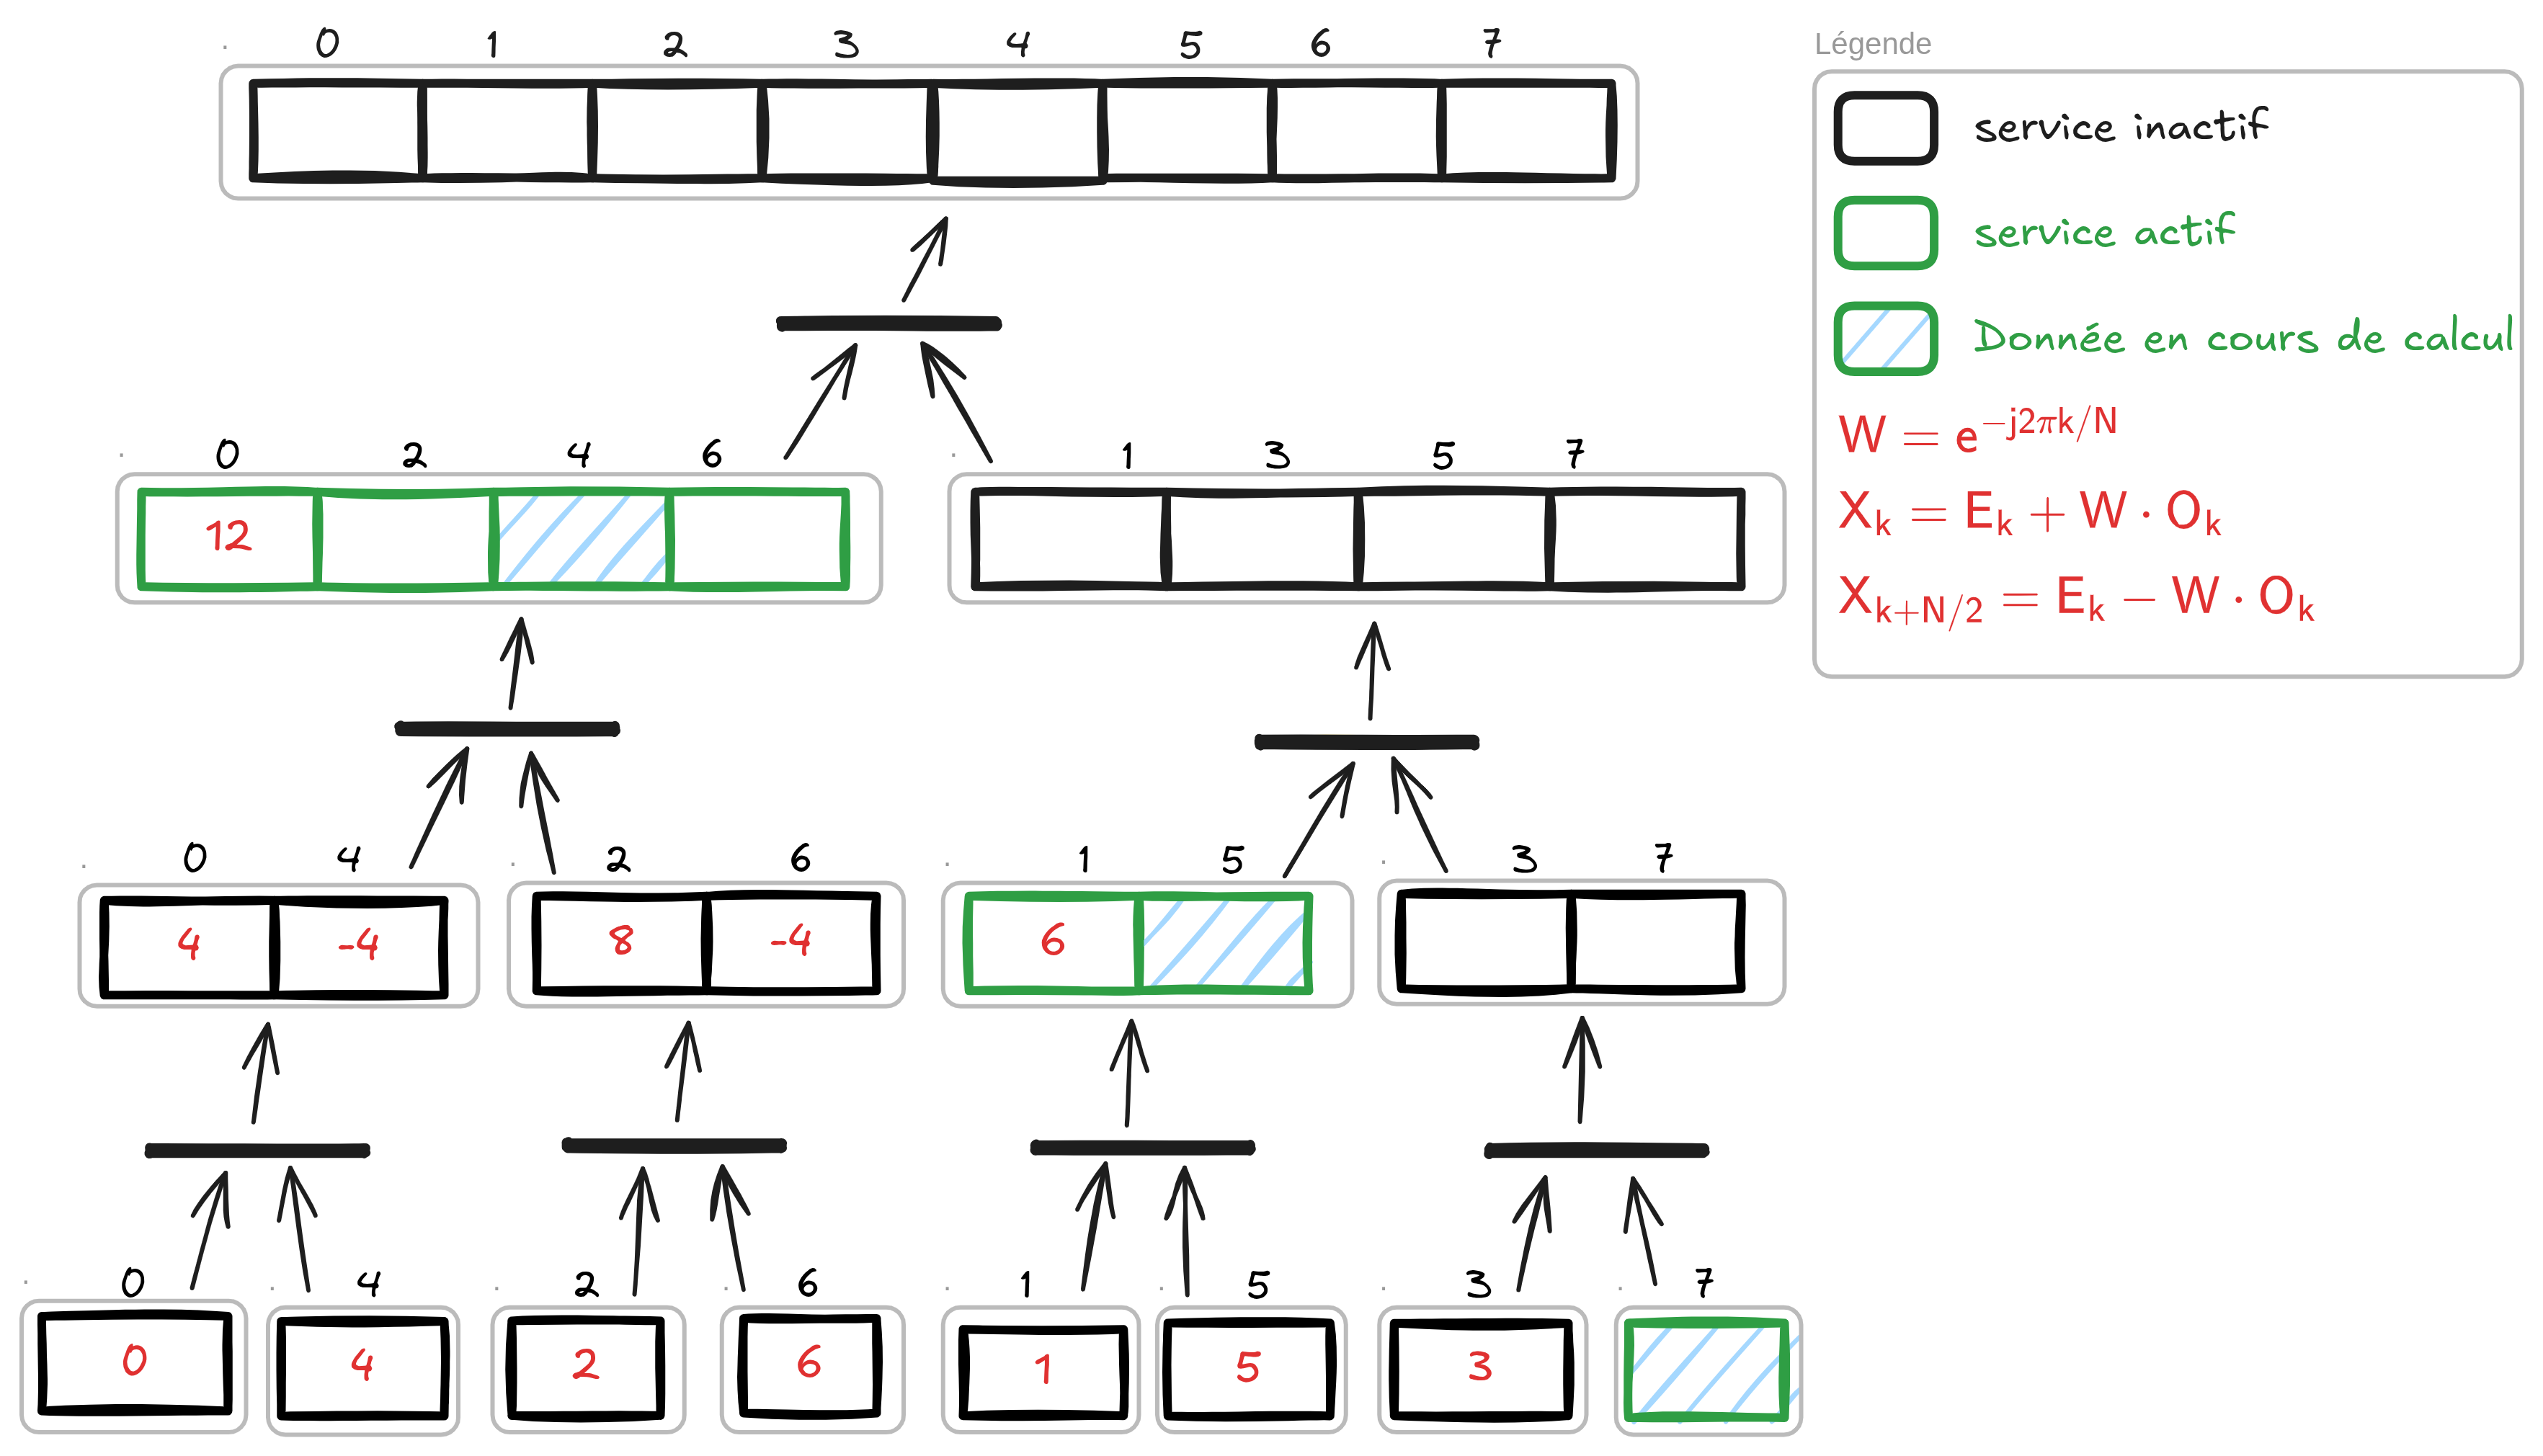
\includegraphics[width=\linewidth]{My-Thesis/Chap3/images/fft no inc-1-1.excalidraw.png}
    \caption{Algorithme non incrémental}
    \label{fig:flow-algo-no-inc}
\end{figure}

À l’inverse, l’approche \textbf{incrémentale} repose sur un découpage explicite des données en blocs. Chaque service peut produire un bloc intermédiaire dès qu’il a reçu deux blocs de ses sous-services. Cela permet une progression locale, incrémentale et asynchrone: les résultats remontent au fur et à mesure qu’ils deviennent disponibles, sans attendre la complétion totale des appels récursifs. Ce mécanisme permet d’exploiter plus finement le parallélisme et d’améliorer la réactivité globale du système.
\begin{figure}[h]
    \centering
    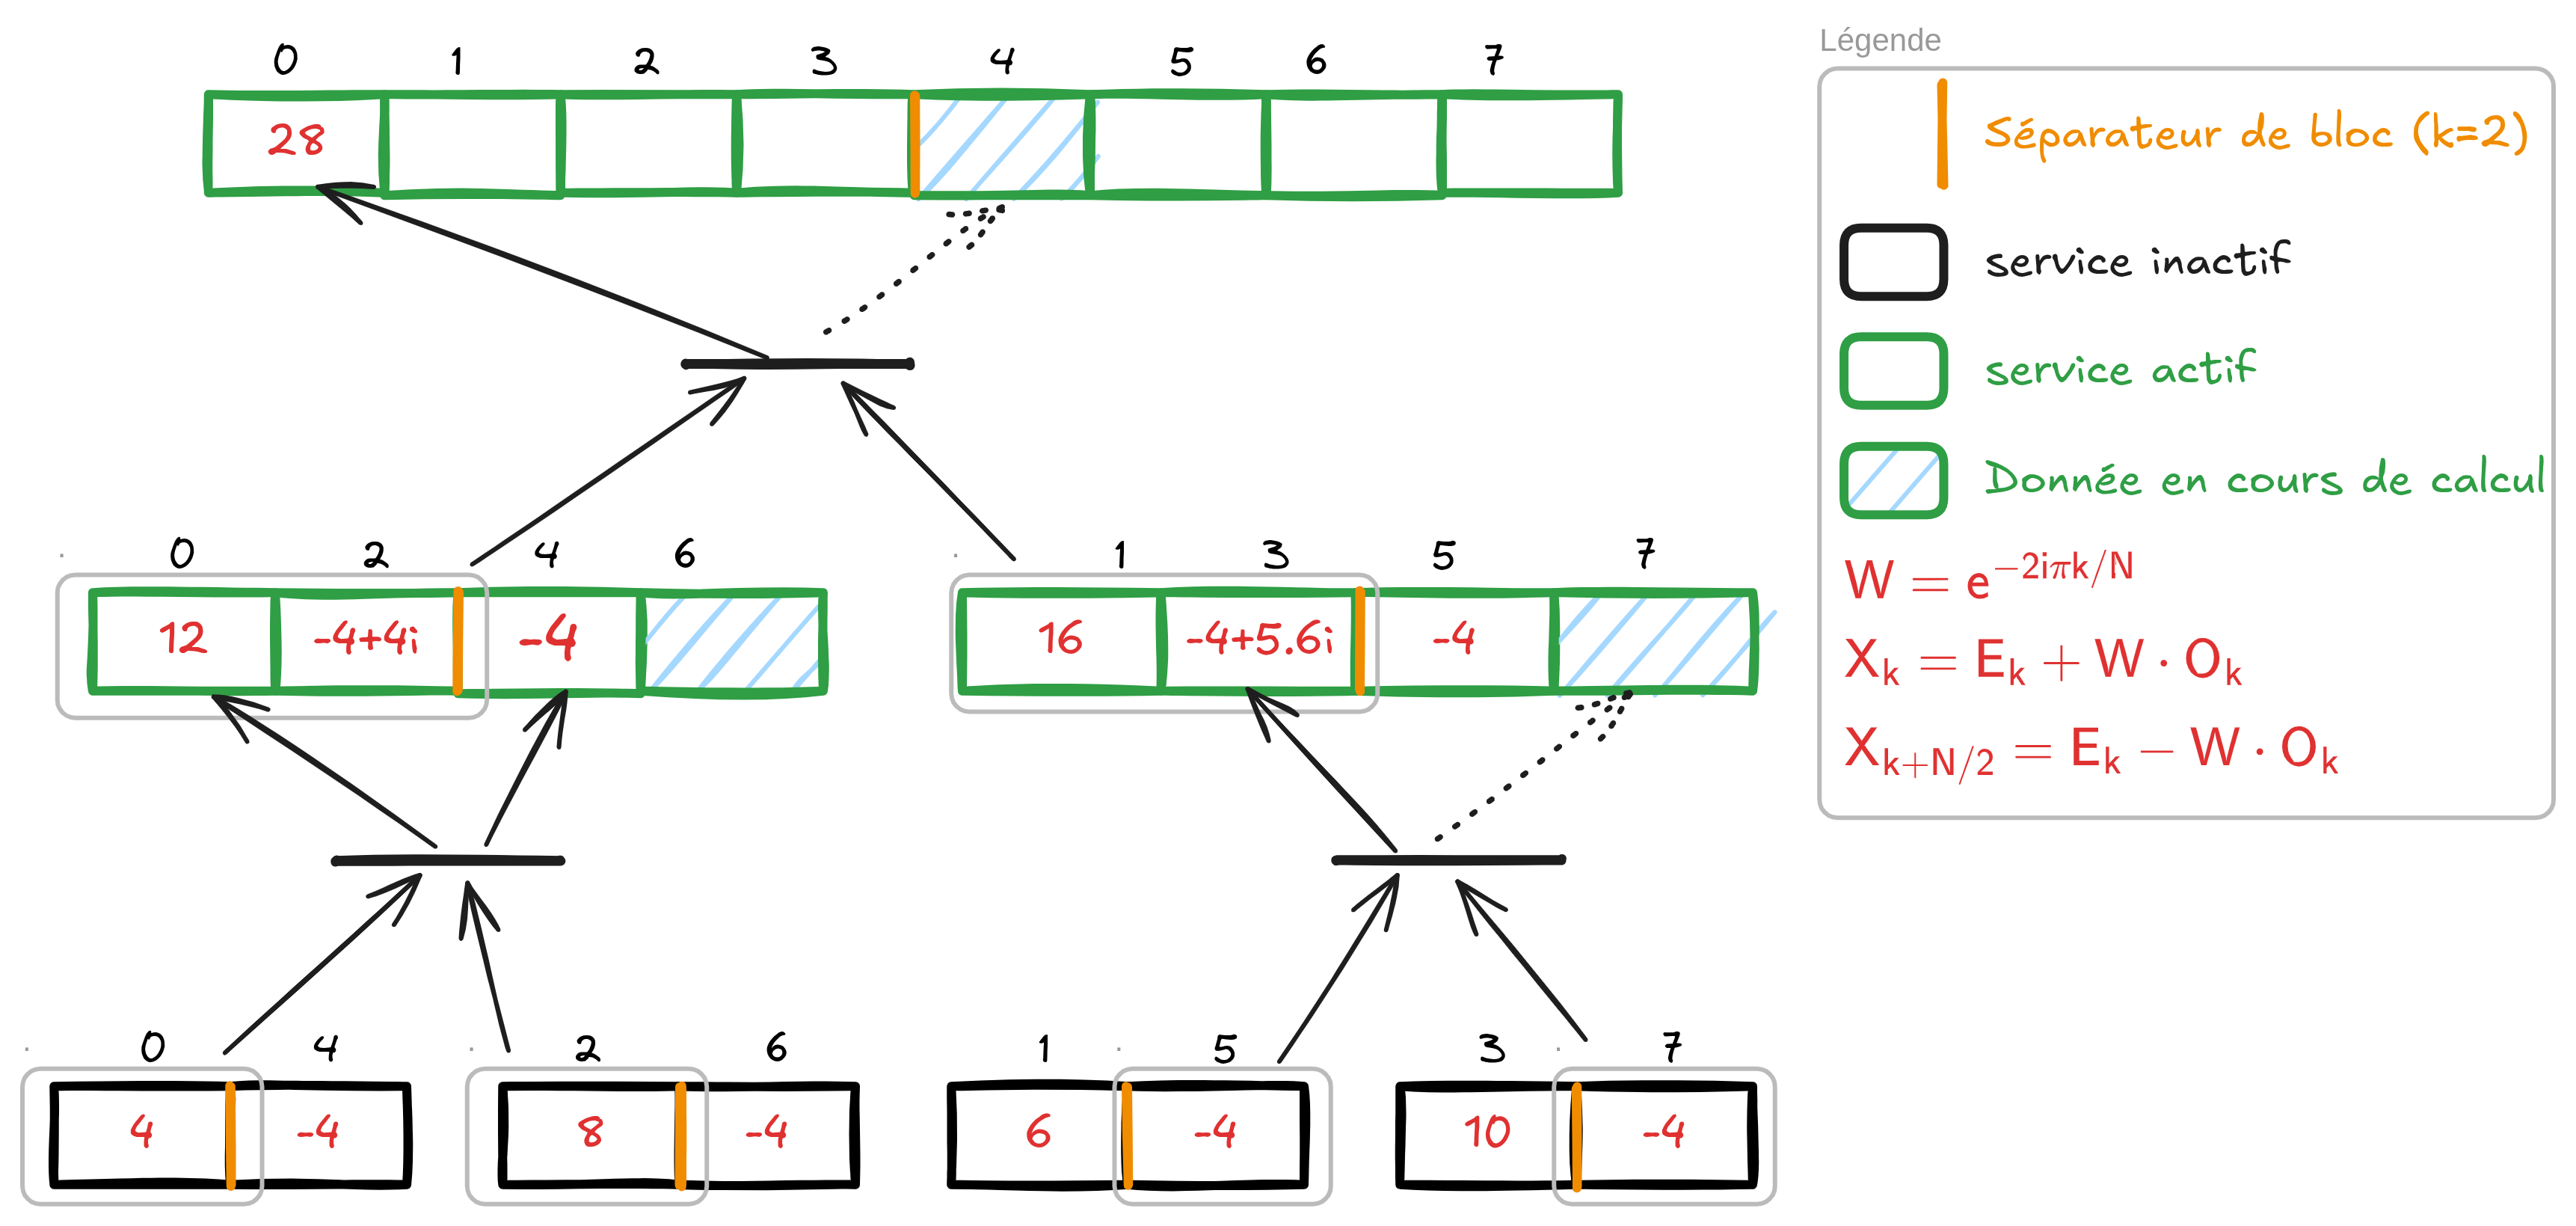
\includegraphics[width=\linewidth]{My-Thesis/Chap3/images/fft inc-k=2-2-1.excalidraw.png}
    \caption{Algorithme incrémental}
    \label{fig:flow-algo-inc}
\end{figure}

Dans cette section, nous comparons ces deux variantes selon plusieurs critères expérimentaux, afin %d’évaluer l’impact de l’incrémentalité sur les performances, la consommation de ressources et le comportement dynamique du système.
d’évaluer la pertinence de la composition incrémentale.

Les figures \ref{fig:flow-algo-no-inc} et \ref{fig:flow-algo-inc} illustrent deux stratégies d’exécution de l’algorithme de la transformée de Fourier rapide (FFT) : une version classique (non incrémentale) et une version incrémentale paresseuse.

La comparaison des différentes approches s’articule autour de trois axes: le \textit{parallélisme}, la \textit{robustesse} et la \textit{latence}.

\textbf{Parallélisme.}
Dans l’approche \textit{non incrémentale} (Figure \ref{fig:flow-algo-no-inc}), le flux d’exécution est rigide et fortement centralisé. Sur tout chemin partant de la racine vers les feuilles, on observe qu’au plus un seul service est actif à un instant donné. Cette exécution suit une structure de type appel récursif, où chaque fonction attend les résultats de ses appels enfants avant de poursuivre. Cette séquentialisation limite fortement les opportunités de parallélisme naturel, sauf à introduire manuellement une orchestration spécifique.

À l’inverse, dans l’approche \textit{incrémentale} (Figure \ref{fig:flow-algo-inc}), l’exécution suit une chaîne de production distribuée. Chaque sous-service peut traiter un fragment de données de manière autonome, puis transmettre un résultat partiel à son parent dès que possible. Cela permet l’activation concurrente de plusieurs services, favorisant ainsi une exécution parallèle fine, contrôlée par les dépendances de données. Cette propriété est inhérente à la sémantique paresseuse et aux mécanismes de synchronisation implicites induits par les GAG.

\textbf{Robustesse.}
Sur le plan de la résilience, l’approche incrémentale présente également des avantages significatifs. Dans l’approche non incrémentale (Figure \ref{fig:flow-algo-no-inc}), un service traite une portion entière de l’entrée et produit son résultat de manière monolithique. Si ce service échoue en cours d’exécution, l’ensemble des données confiées est perdu, et le calcul doit redémarrer depuis le début ou un point de reprise explicitement programmé.

Dans l’approche incrémentale, au contraire, les données sont traitées par \textbf{blocs}. Lorsqu’un service échoue, il se peut qu’il ait déjà fourni une partie de ses résultats à son parent. On ne perd alors qu’une portion limitée du travail, ce qui rend le système plus robuste face aux défaillances. Cette \textbf{tolérance partielle} aux pannes est une propriété précieuse dans des environnements distribués et potentiellement instables.

\textbf{Latence de résultat.}
En mode incrémental, dès qu’un fragment de données est prêt, il peut être immédiatement transmis au niveau supérieur, permettant une réduction de la latence. L’approche non incrémentale, elle, ne produit aucun résultat tant que l’ensemble du traitement n’est pas achevé, ce qui allonge le temps de réponse dans les systèmes interactifs.

Ces deux figures permettent de visualiser clairement les différences fondamentales entre les deux approches. 
Le tableau~\ref{tab:comparaison-approches} résume les principales différences entre les deux approches selon les trois axes étudiés.
\begin{table}[H]
\centering
\caption{Comparaison entre l’approche non incrémentale et l’approche incrémentale}
\label{tab:comparaison-approches}
\begin{tabular}{|p{3cm}|p{5.2cm}|p{5.2cm}|}
\hline
\textbf{Critère} & \textbf{Approche non incrémentale} & \textbf{Approche incrémentale} \\ \hline
\textbf{Parallélisme} 
& Flux d’exécution séquentiel et centralisé.  
Un seul service actif par chemin.  
Peu de parallélisme naturel. 
& Flux distribué sous forme de chaîne de production.  
Plusieurs services peuvent travailler en parallèle grâce à la distribution des dépendances. \\ \hline

\textbf{Robustesse}
& Échec d’un service égale perte complète du travail sur la portion traitée.  
Redémarrage global souvent nécessaire.
& Tolérance partielle aux pannes : seules les parties non transmises sont perdues.  
Reprise locale facilitée. \\ \hline

\textbf{Latence des résultats}
& Les résultats sont produits uniquement à la fin du traitement complet. 
& Résultats partiels transmis dès qu’ils sont disponibles, réduisant la latence globale. \\ \hline

% \textbf{Complexité}
% & Gestion simple mais peu flexible. 
% & Coordination plus complexe (gestion des dépendances, synchronisation), mais plus flexible. \\ \hline
\end{tabular}
\end{table}


L’approche incrémentale, en s’appuyant sur une exécution paresseuse distribuée, offre des avantages majeurs en termes de parallélisme, robustesse et flexibilité, au prix d’une complexité accrue de coordination et d’une gestion fine des dépendances. Ces caractéristiques en font un candidat idéal pour les systèmes modernes orientés services.

\mySection{Conclusion}{}
Dans ce chapitre, nous avons présenté une expérimentation visant à évaluer la pertinence et l’efficacité de la composition incrémentale des services dans un contexte distribué, à travers l’implémentation d’un algorithme paresseux de la transformée de Fourier Rapide (FFT).
Ce chapitre a démontré la faisabilité de la composition incrémentale basée sur les GAG dans un contexte réel d’algorithme intensif (FFT). Il a permis de valider expérimentalement la réduction de latence, l’augmentation du parallélisme et la flexibilité de l’approche par rapport à une exécution classique. Ces résultats renforcent l’intérêt d’une orchestration pilotée paresseusement, et ouvrent des perspectives d’amélioration du moteur GAG et d’élargissement à d’autres classes d’algorithmes.
